\section{Diagnostics and further results}
\label{app:diag}
\paragraph{Proofs of Propositions 1 and 2.}
Assumptions are those of Sec.~\ref{sec:theory}: i.i.d.\ labelled and unlabelled records, $\mathrm{Var}(Y)<\infty$, $\mathrm{Var}(g(W))\in(0,\infty)$.
\emph{Variance.} The labelled and unlabelled records are independent, so
$\mathrm{Var}(\hat\theta_{g,\lambda})=\mathrm{Var}(Y-\lambda g)/n+\lambda^2\mathrm{Var}(g)/N
=\tfrac1n\{\mathrm{Var}(Y)-2\lambda\mathrm{Cov}(Y,g)+\lambda^2(1+\rho)\mathrm{Var}(g)\}$.
This is a convex quadratic in $\lambda$, minimised at $\lambda^\star=\mathrm{Cov}(Y,g)/\{(1+\rho)\mathrm{Var}(g)\}$, where it equals $\tfrac{\mathrm{Var}(Y)}n\{1-R_g^2/(1+\rho)\}$ (Eq.~\ref{eq:var}).
\emph{Proposition 1.} A Wald interval has half-width proportional to the estimated standard deviation, which is consistent for the square root of the variance above, so by Slutsky's theorem the ratio of two widths converges to the ratio of the square roots of the minimal variances; with Eq.~\eqref{eq:var} for $g_1,g_2$ the common factor $\mathrm{Var}(Y)/n$ and the quantile cancel.
\emph{Proposition 2.} Write $m=\mathbb E[Y\mid W]$ and $V=\mathrm{Var}(m)$, so $\mathrm{Var}(Y)=\mathbb E\,\mathrm{Var}(Y\mid W)+V$ (the term $\mathrm{Var}(Y\mid W)$ in the statement is its expectation). Since $g$ is a function of $W$, $\mathrm{Cov}(Y,g)=\mathrm{Cov}(m,g)$, hence $R_g^2=\mathrm{corr}^2(m,g)\,\eta^2\le\eta^2$ by Cauchy--Schwarz, with equality iff $g$ is almost surely an affine function of $m$.
Substituting $\eta^2$ in Eq.~\eqref{eq:var}: $\mathrm{Var}^\star(g)\ge\tfrac1n\{\mathrm{Var}(Y)-\tfrac{V}{1+\rho}\}=\tfrac1n\{\mathbb E\,\mathrm{Var}(Y\mid W)+\tfrac{\rho}{1+\rho}V\}$, and $\tfrac{\rho}{n(1+\rho)}=\tfrac1{n+N}$ gives the second form. \qed
We do not reprove the statement that the bound is the semiparametric efficiency bound; it is cited as known \citep{angelopoulos2023ppiplus}.

\paragraph{Population headroom per pool and class.}
Table~\ref{tab:headroom} gives the numbers behind Fig.~\ref{fig:headroom} (asymptotic width ratio to PPI++, mean $\pm$ SD over ten 2-fold splits).

\begin{table}[h]
\caption{Asymptotic CI-width ratio to power-tuned PPI++ ($N\to\infty$; 1 = parity, $<1$ narrower) per pool and control-variate class; mean $\pm$ SD over ten random 2-fold cross-fitting splits. ``--'': no features $X$ in the pool.}
\label{tab:headroom}
\centering
\scriptsize\setlength{\tabcolsep}{3pt}\begin{tabular}{lrrrrrr}
\toprule
pool & PPI & lin.\ $f$ & isot.\ $f$ & GBM $f$ & lin.\ $(f,X)$ & GBM $(f,X)$ \\
\midrule
galaxies & $1.000{\pm}.000$ & $1.000{\pm}.000$ & $1.003{\pm}.001$ & $1.008{\pm}.002$ & -- & -- \\
forest & $1.003{\pm}.000$ & $1.002{\pm}.002$ & $1.004{\pm}.005$ & $1.021{\pm}.011$ & -- & -- \\
alphafold & $1.001{\pm}.000$ & $1.000{\pm}.000$ & $0.999{\pm}.001$ & $1.003{\pm}.002$ & -- & -- \\
gene\_expression & $1.106{\pm}.000$ & $1.000{\pm}.000$ & $0.988{\pm}.000$ & $0.989{\pm}.001$ & -- & -- \\
census\_income & $1.022{\pm}.000$ & $1.000{\pm}.000$ & $0.998{\pm}.000$ & $0.998{\pm}.000$ & $0.999{\pm}.000$ & $0.995{\pm}.000$ \\
census\_healthcare & $1.000{\pm}.000$ & $1.000{\pm}.000$ & $1.000{\pm}.000$ & $1.000{\pm}.000$ & $1.000{\pm}.000$ & $1.000{\pm}.000$ \\
census\_education & $1.000{\pm}.000$ & $1.000{\pm}.000$ & $1.000{\pm}.000$ & $1.000{\pm}.000$ & $1.000{\pm}.000$ & $0.999{\pm}.000$ \\
\bottomrule
\end{tabular}

\end{table}

\paragraph{Label shift (\texttt{plankton}).}
The predictor is binary. Without shift (labelled and unlabelled drawn from the 2013 pool, $N=10^4$, 2000 repetitions) the like-for-like ratio of the cross-fitted affine and isotonic adjusters is 1.215 and 1.267 at $n=25$, 1.039 at $n=100$ and 1.003 at $n=1000$, and PPI++ covers 0.856, 0.911 and 0.943 at those sizes: the same picture as Sec.~\ref{sec:real}.
Under the stress test (labelled from 2013, unlabelled from 2014, truth the 2014 mean of $Y$), the exchangeability assumption fails: PPI++ covers 0.741 at $n=100$, 0.607 at $n=200$ and 0.349 at $n=1000$, the two adjusters 0.768/0.768, 0.622/0.624 and 0.352/0.358, and the labelled-only interval 0.000 at $n=1000$.
PPI with $\lambda=1$ covers 0.952, 0.944 and 0.946 at the same sizes; we did not isolate why, but it is consistent with power-tuning shifting weight toward the biased labelled mean. In this regime a shorter interval is not a saving because no interval tested is valid; we have no remedy.

\paragraph{Unlabelled records without outcomes (\texttt{ballots}).}
Only the 1027 labelled ballots have a truth, so two diagnostics are run. \emph{Subsample}: $n$ labelled drawn without replacement from the 1027 and the rest as unlabelled; truth is the 1027-ballot mean. Coverage is 0.98 to 1.00 for PPI++ at $n\ge25$ (the finite population fixes the truth; this is not a validity test of the i.i.d.\ theory) and the adjusters are 0.0\% to 2.2\% wider.
\emph{Width only}: unlabelled are the $78{,}150$ ballots with predictions only. The isotonic adjuster is 2.4\%, 2.1\%, 1.7\%, 1.2\% and 0.6\% wider than PPI++ at $n=25,50,100,200,400$, and the labelled-only interval is 5.0 to 11 times wider. No coverage is claimed.

\paragraph{Further figures.}\label{app:figs}
Figures~\ref{fig:app_c2}--\ref{fig:app_named_b} extend Figs.~\ref{fig:c2} and~\ref{fig:c3} and follow the same layout (paired like-for-like width ratio above, coverage below).
\begin{figure}[h]
\centering
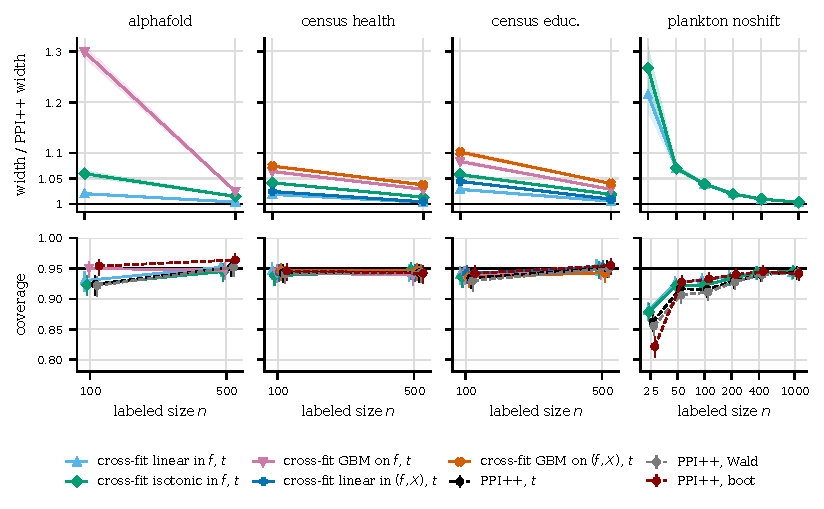
\includegraphics[width=\linewidth]{figures/fig_c2_real_app_a.pdf}
\caption{Mean estimation on \texttt{alphafold}, \texttt{census\_healthcare}, \texttt{census\_education} ($n=100,500$, 1000 repetitions) and on \texttt{plankton} without shift ($n$ from 25 to 1000, 2000 repetitions).}
\label{fig:app_c2}
\end{figure}
\begin{figure}[h]
\centering
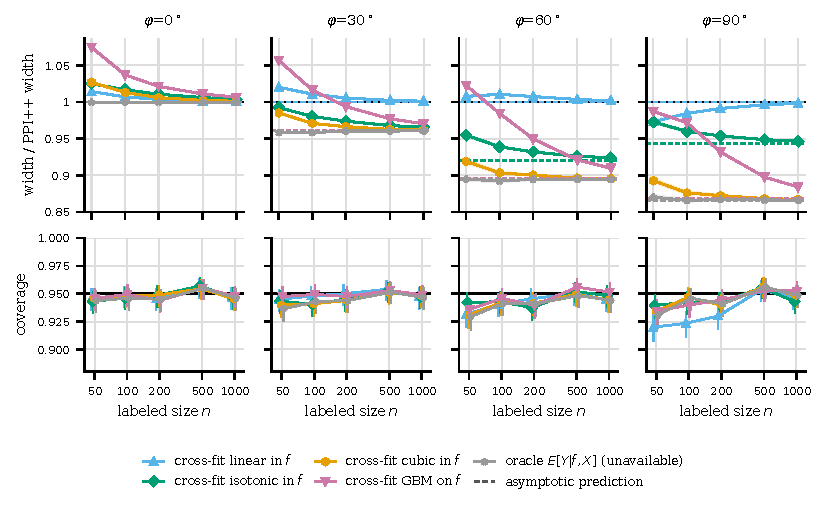
\includegraphics[width=\linewidth]{figures/fig_c3_synth_app_knob_rho1.pdf}
\caption{Knob family at $\rho=1$ ($N=n$), 2000 repetitions per cell.}
\label{fig:app_knob1}
\end{figure}
\begin{figure}[h]
\centering
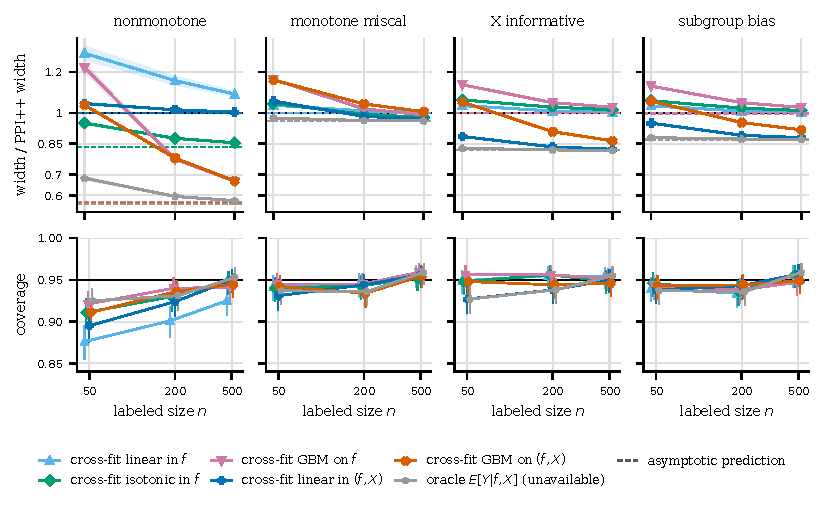
\includegraphics[width=\linewidth]{figures/fig_c3_synth_app_named_a_rho0.1.pdf}
\caption{\texttt{nonmonotone}, \texttt{monotone\_miscal}, \texttt{X\_informative}, \texttt{subgroup\_bias} at $\rho=0.1$, 1000 repetitions per cell, with the $(f,X)$ adjusters.}
\label{fig:app_named_a}
\end{figure}
\begin{figure}[h]
\centering
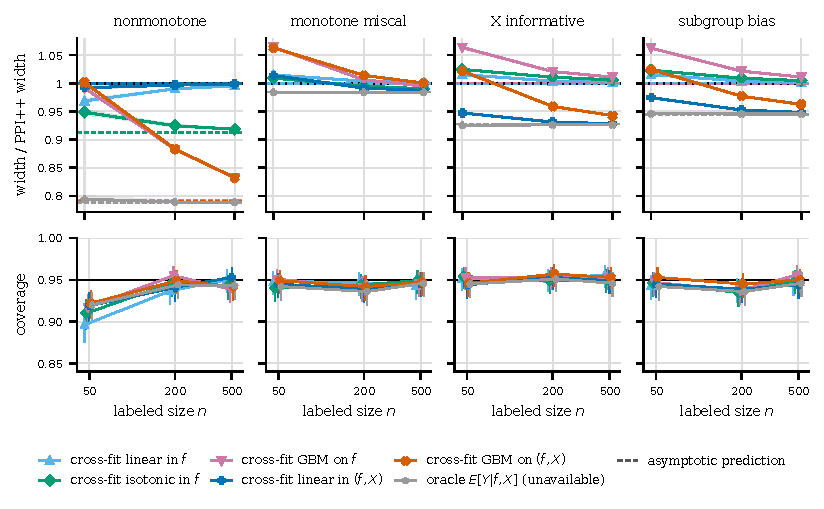
\includegraphics[width=\linewidth]{figures/fig_c3_synth_app_named_a_rho1.pdf}
\caption{As Fig.~\ref{fig:app_named_a} at $\rho=1$.}
\end{figure}
\begin{figure}[h]
\centering
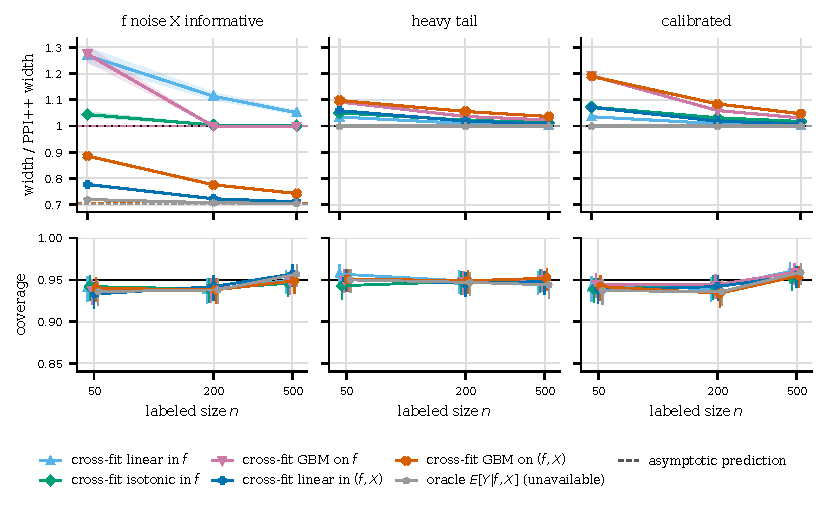
\includegraphics[width=\linewidth]{figures/fig_c3_synth_app_named_b_rho0.1.pdf}
\caption{\texttt{f\_noise\_X\_informative}, \texttt{heavy\_tail}, \texttt{calibrated} at $\rho=0.1$, 1000 repetitions per cell.}
\label{fig:app_named_b}
\end{figure}
\begin{figure}[h]
\centering
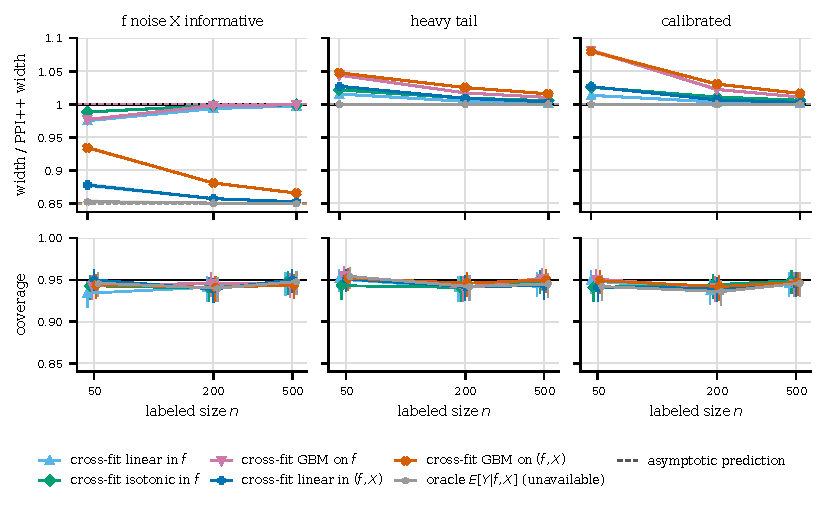
\includegraphics[width=\linewidth]{figures/fig_c3_synth_app_named_b_rho1.pdf}
\caption{As Fig.~\ref{fig:app_named_b} at $\rho=1$.}
\end{figure}
